
%%%%%%%%%%%%%%%%%%%%%%% file typeinst.tex %%%%%%%%%%%%%%%%%%%%%%%%%
%
% This is the LaTeX source for the instructions to authors using
% the LaTeX document class 'llncs.cls' for contributions to
% the Lecture Notes in Computer Sciences series.
% http://www.springer.com/lncs       Springer Heidelberg 2006/05/04
%
% It may be used as a template for your own input - copy it
% to a new file with a new name and use it as the basis
% for your article.
%
% NB: the document class 'llncs' has its own and detailed documentation, see
% ftp://ftp.springer.de/data/pubftp/pub/tex/latex/llncs/latex2e/llncsdoc.pdf
%
%%%%%%%%%%%%%%%%%%%%%%%%%%%%%%%%%%%%%%%%%%%%%%%%%%%%%%%%%%%%%%%%%%%


\documentclass[runningheads,a4paper]{llncs}

\usepackage{amssymb}
\setcounter{tocdepth}{3}
\usepackage{subcaption}
\captionsetup{compatibility=false}
\usepackage{booktabs}
\usepackage{graphicx}
\usepackage{epstopdf}
\usepackage[utf8]{inputenc}
\usepackage[T1]{fontenc}
\usepackage{lmodern}

\usepackage{url}
\urldef{\mailsa}\path|loic.tetrel@mail.mcgill.ca|    
\newcommand{\keywords}[1]{\par\addvspace\baselineskip
\noindent\keywordname\enspace\ignorespaces#1}

\begin{document}

\mainmatter  % start of an individual contribution

% first the title is needed
\title{Assignment 2 : Eigenfaces for Face Recognition}

% a short form should be given in case it is too long for the running head
\titlerunning{Assignment 2 : Eigenfaces for Face Recognition}

% the name(s) of the author(s) follow(s) next
%
% NB: Chinese authors should write their first names(s) in front of
% their surnames. This ensures that the names appear correctly in
% the running heads and the author index.
%
\author{Loïc Tetrel}
%loic.tetrel@mail.mcgill.ca
\authorrunning{Assignment 2 : Eigenfaces for Face Recognition}
% (feature abused for this document to repeat the title also on left hand pages)

% the affiliations are given next; don't give your e-mail address
% unless you accept that it will be published
\institute{McGill University\\
845 Rue Sherbrooke O, QC H3A 0G4, Montréal, Canada\\
\mailsa\\
}

%\toctitle{Sensorless registration of echographic images for 3D ultrasound}
\maketitle

%\begin{abstract}

\section{Introduction}

The use of principal component analysis has been widely use in the area of computer vision. 
In this assignment we will investigate it use for face recognition. 
Because the dimension of such point is really big ($393216$ dimensions point for image $512\times768$), the main idea is to project the image into a sublower space called ``face-space'' that best encodes the variation among known face images \cite{sirovich1987low} and it is derived from the Fourier transform. 
Each $M$ image characterized by $[1,N^2]$ with $N^2$ dimensions differs from the average $\Psi=\frac{1}{M}\sum_{n=1}^M\Gamma_n$ by the matrix $A=\Gamma-\Psi$. 
Principal component analysis will find the $M$ orthogonal vectors $v_M$ that maximizes the variance $\lambda_k$ along each vector, i.e. we search the eigen vectors $v_k$ and eigen values $\lambda_k$ of the covariance matrix $C$ :
\begin{equation}
C=A^tA
\end{equation}
Because the covariance $C$ is $N^2$ by $N^2$, the snapshot method \cite{turk1991face} says that the best $\lambda_k$ are the same as $C=AA^t$ which is $M$ by $M$. 
Usually the training set is much lower than the number of dimension $(M<<N^2)$ so this allowed us to compute $v_M$ and $\lambda_k$ much faster. The mapping from the pixel-space to the face-space and is given by :
\begin{equation}
u=v^tA
\end{equation}

The matrix $u$ is called the eigen faces and is $M$ by $N^2$.

\section{Principal component analysis for subject classification}

The FERET database \cite{phillips1998feret} is used in this assignment. The pose nomenclature is wrong and all the r* will have reverse angles values, re is $+80^{\circ}$. 
I will use $28$ images for all the $52$ subjects for the training, and $4$ images for the testing.

\subsection{Results of principal component analysis}

The mean image of the FERET are shown in Fig.\ref{fig:mean_face}.Looking at the eigen faces (Fig. \ref{fig:10_eigen_faces}), it can be seen that the first eigen vector looks like a human face. However there is no information about the hairs, represented by $u_5$ or $u_8$. The last faces are very dark and there isn't a lot of information coming from it.

\begin{figure}
\centering

\includegraphics[height=1.5cm]{Figures/mean_face}
\caption{Mean face of the training set.}
\label{fig:mean_face}
\end{figure}



\begin{figure}
\centering
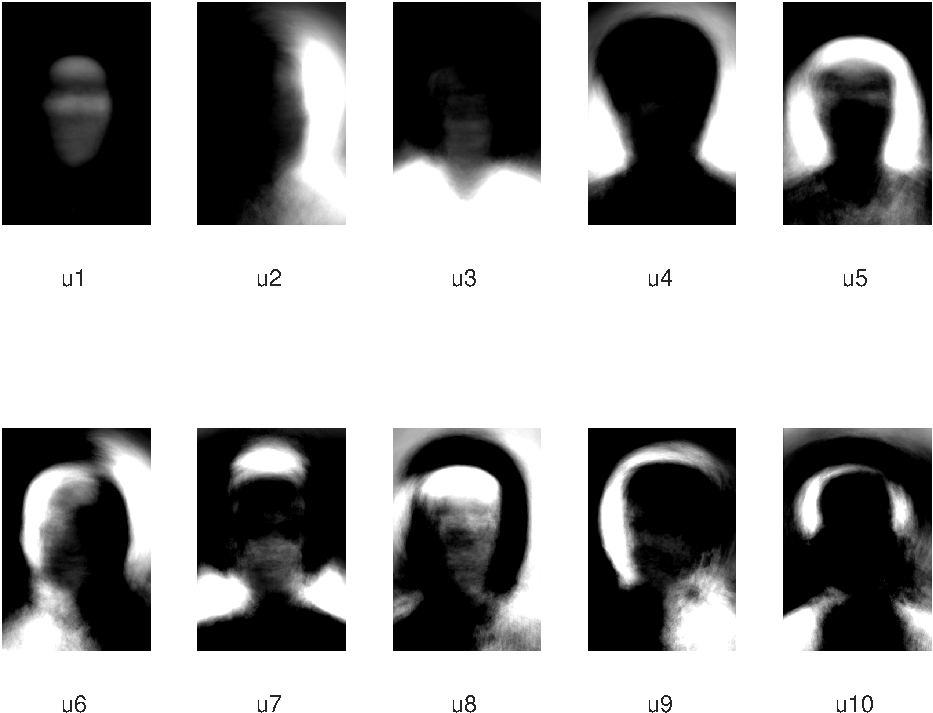
\includegraphics[height=5cm]{Figures/10_eigen_faces}
\caption{The $10$ first eigen spaces.}
\label{fig:10_eigen_faces}
\end{figure}

\subsection{Reconstruction}

One way to evaluate the number of dimensions used in our new space is to (re)project the images in the pixel space using a fewer dimension. Then the reconstruction error can be computed between the truth image $\Gamma_{t}$ and the projected image $\Gamma_p$ :

\begin{equation}
Rec_{error}=\sum_M (\sqrt{\sum_{N^2}(\Gamma_{t}-\Gamma_p)^2})
\end{equation}

Obviously, the more we use eigen values, the more accurate we are. Taking into account the future computational time, it is more interesting to take less eigen values like $50$ which give an accuracy of  $1\%$ not far from the standard $5\%$ (Fig. \ref{fig:error_rec_eig}). It is also interesting to see the importance of each eigen values. The Figure \ref{fig:rec_eig_face} shows qualitatively the accuracy for $3$ random images from the training set with $1,5,10,20,50$ eigen values, and we see that using just a few eigen faces does not produce good results.

\begin{figure}
\centering
    \begin{subfigure}[b]{0.4\textwidth}
      \centering
	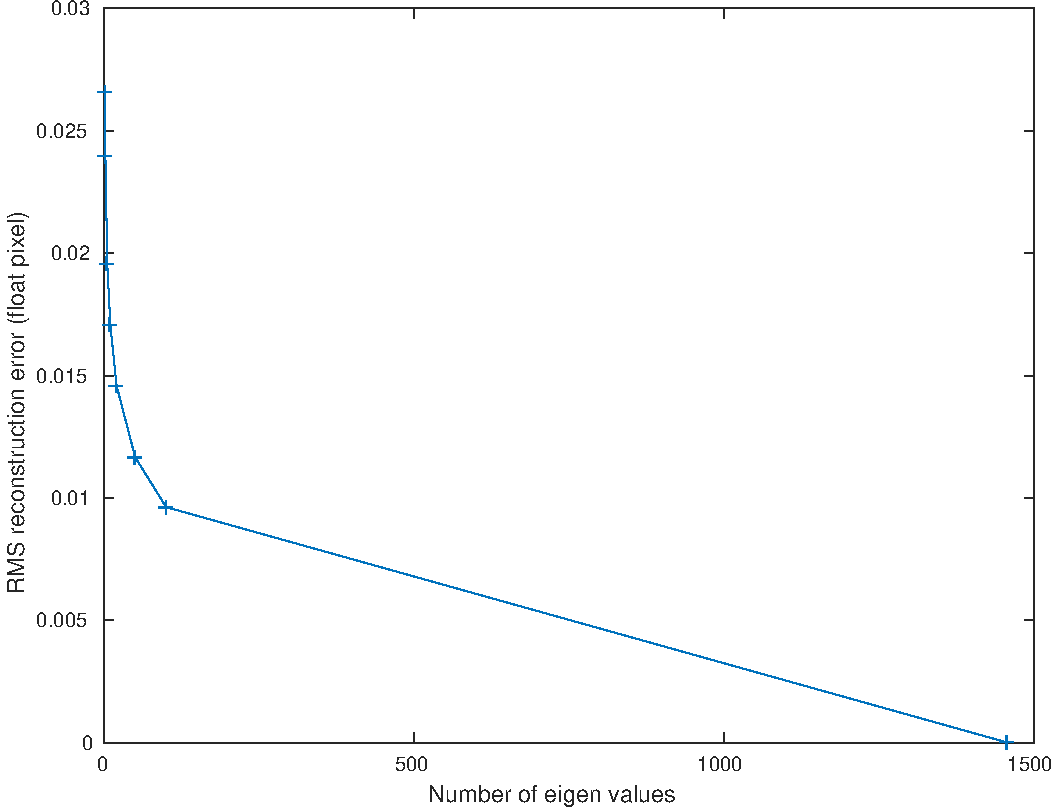
\includegraphics[height=2.5cm]{Figures/error_rec_eig}
	\caption{}
    \end{subfigure}~
\begin{subfigure}[b]{0.4\textwidth}
      \centering
      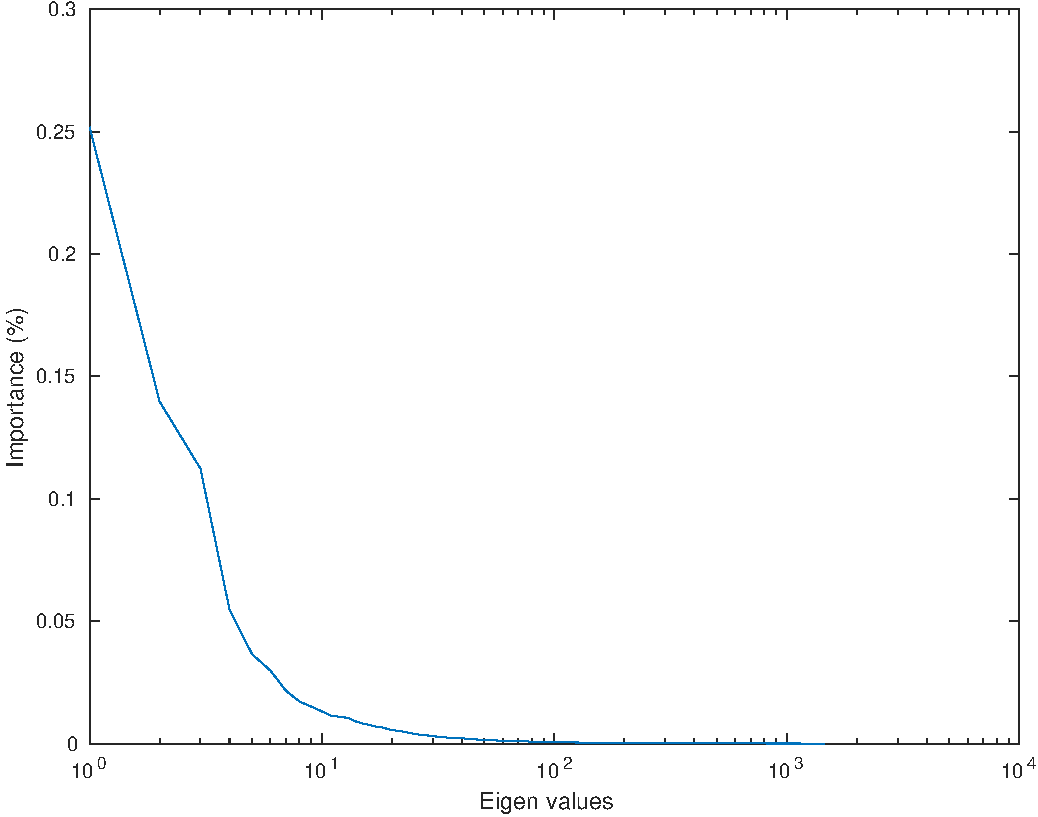
\includegraphics[height=2.5cm]{Figures/importance_eigen}
      \caption{}
    \end{subfigure}~
\caption{(a) RMS error reconstruction versus number of eigen values. (b) Importance of the eigen values.}
\label{fig:error_rec_eig}
\end{figure}



\begin{figure}
\centering
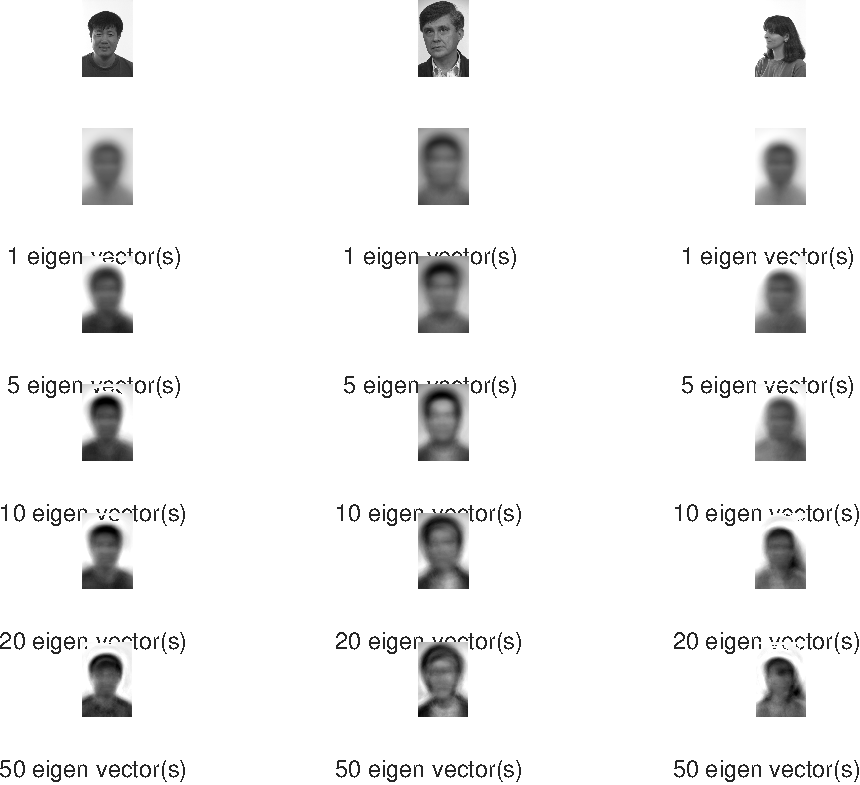
\includegraphics[height=5cm]{Figures/rec_eig_face}
\caption{RMS error reconstruction versus number of eigen values.}
\label{fig:rec_eig_face}
\end{figure}

\subsection{Classification and recognition}

The classification with eigen faces can be done using a nearest neighbour algorithm. The classification for one image $\Gamma$ is the label $k$ if the nearest image of $\Gamma$ is a subject $k$. The distance between images $d_{\Gamma_{ij}}$ is define as the norm of the eigen weights $w=Au'$.

\begin{equation}
d_{\Gamma_{ij}}=\|w_i-w_j\|
\end{equation}

The error decrease with the number of eigen values. The optimal number of eigen values seem to be at minimum $20$, because the error start to be constant at $30\%$ with this value \ref{fig:error_rate_eig}. The error min is given for $50$ eigen values.

\begin{figure}
\centering
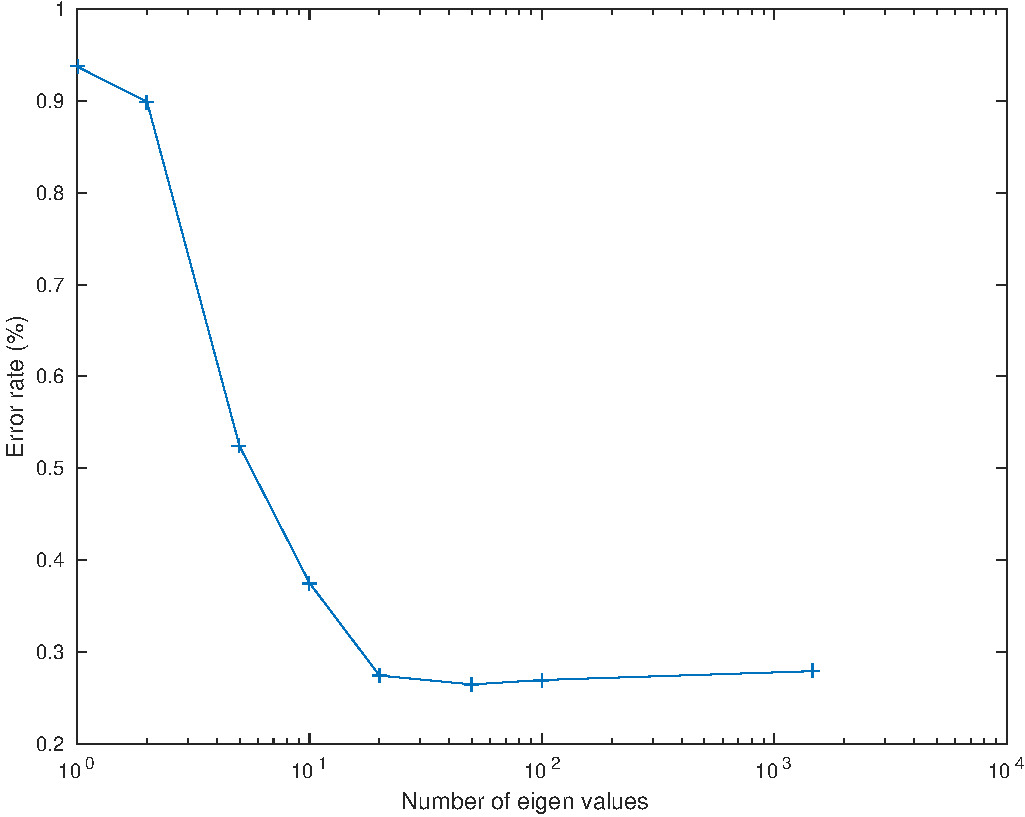
\includegraphics[height=2.5cm]{Figures/error_rate_eig}
\caption{Error recognition rate.}
\label{fig:error_rate_eig}
\end{figure}

The Figure \ref{fig:error_class_eig} shows three missclassified images and three good classification. We wee that even for a human the missclassified images are not obvious.

\begin{figure}
\centering
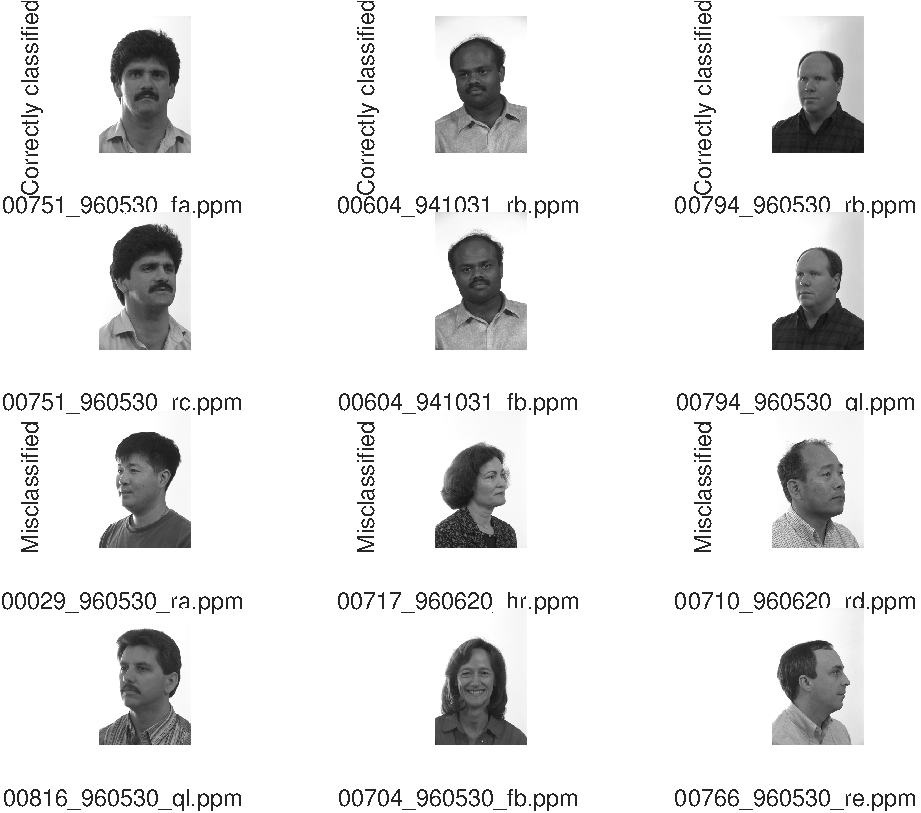
\includegraphics[height=5cm]{Figures/error_class_eig}
\caption{Missclassified and good classified examples.}
\label{fig:error_class_eig}
\end{figure}

\subsection{Probabilistic Face Recognition}

The classification can be also computed using a bayesian rule. Assuming that the data $d$ (pixels) are well fitted to the model $m$ (eigen values), the probability for one class $l$ given an image $I$ is :

\begin{equation}
p(l=k|I)=\frac{p(I|l=k)~p(l=k)}{p(I)}
\end{equation}

Because $p(l=k|I) ~\alpha~p(I|l=k)p(l=k)$, to assign a label to a given image we will assume the following assumption :

\begin{equation}
\max p(l=k|I) \simeq \max p(I|l=k)
\end{equation}

The likelihood $p(I|l=k)$ for each subject $k$ will be approximated by a multivariate gaussian on $28$ images for each subject with $50$ eigen weights with the covariance $\Sigma$ $50$ by $50$ and mean $\mu$. Using $50$ values, the recognition rate is $60\%$ which is lower than $75\%$ for the nearest neighbour and I think this is due to the number of the training. When we take not enough training data, the eigen weights are not well distributed and there are computation problem with the covariance. The Figure \ref{fig:proba_eig} shows the distribution of the previous images of Figure \ref{fig:error_class_eig}.

\begin{figure}
\centering
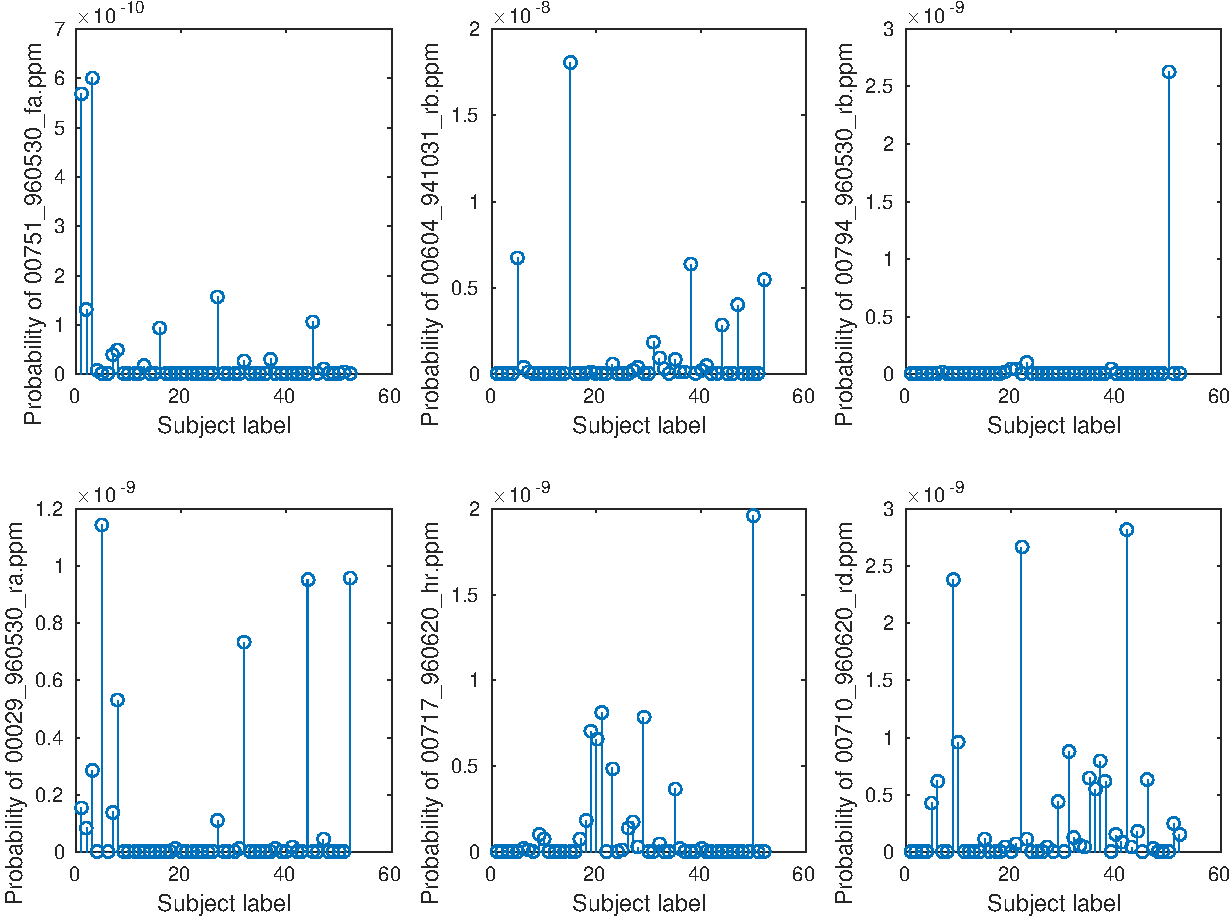
\includegraphics[height=2.5cm]{Figures/proba_eig}
\caption{Likelihoods of missclassified and good classified examples.}
\label{fig:proba_eig}
\end{figure}

\section{Principal component analysis for pose classification}

In this section, we want to classify the pose of each subject. We will map poses to seven coarse pose class $\Theta=[ -90^{\circ},-50^{\circ},-15^{\circ},0^{\circ},+15^{\circ},+50^{\circ}+90^{\circ}]$. $90\%$ of the data will be used  for training and $10\%$ will be used for testing.

\subsection{Results of principal component analysis for pose classification}

The mean image of each pose class are shown in Fig.\ref{fig:mean_image_pose}. The 10 first eigen faces for each pose class are shown in Figure \ref{fig:10_eigen_faces_pose}. We can see that the eigen faces follows well the angles.

\begin{figure}
\centering
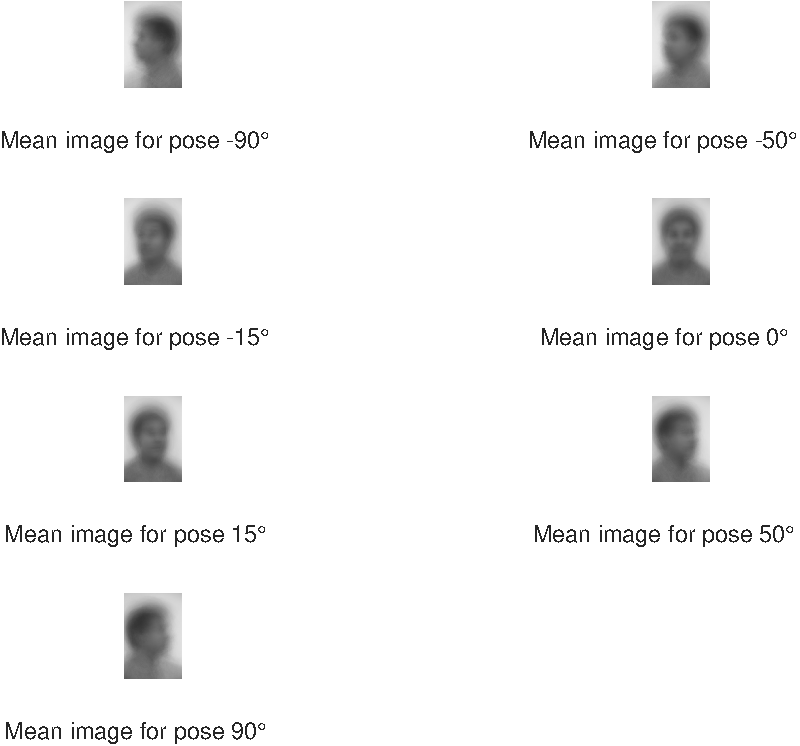
\includegraphics[height=5cm]{Figures/mean_image_pose}
\caption{Mean face of each pose of the training set.}
\label{fig:mean_image_pose}
\end{figure}

\begin{figure}
\centering
\begin{subfigure}[b]{0.4\textwidth}
	\centering
	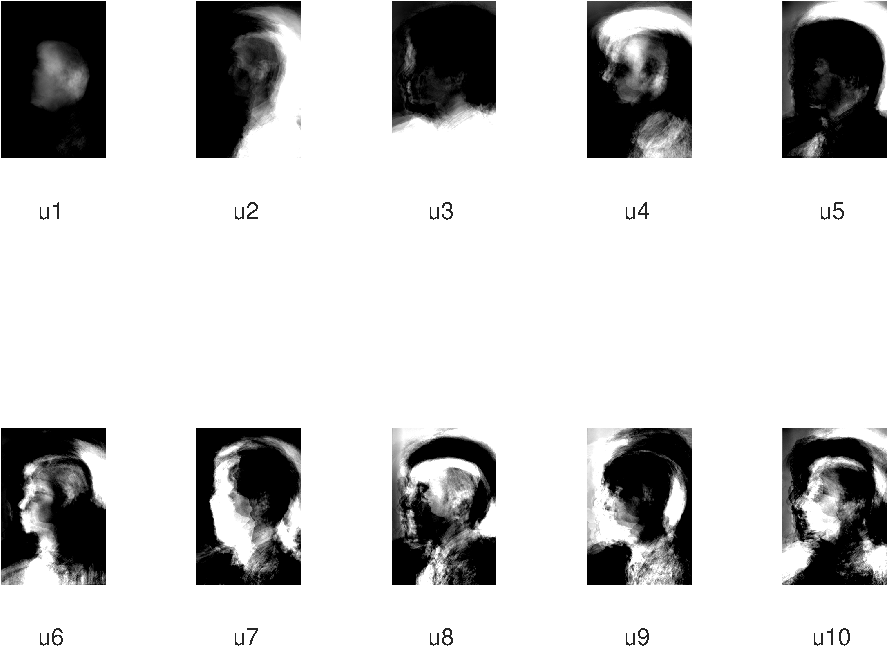
\includegraphics[height=2.5cm]{Figures/10_eigen_faces_m90deg}
\caption{$\Theta_1= -90^{\circ}$}
\end{subfigure}~
\begin{subfigure}[b]{0.4\textwidth}
	\centering
	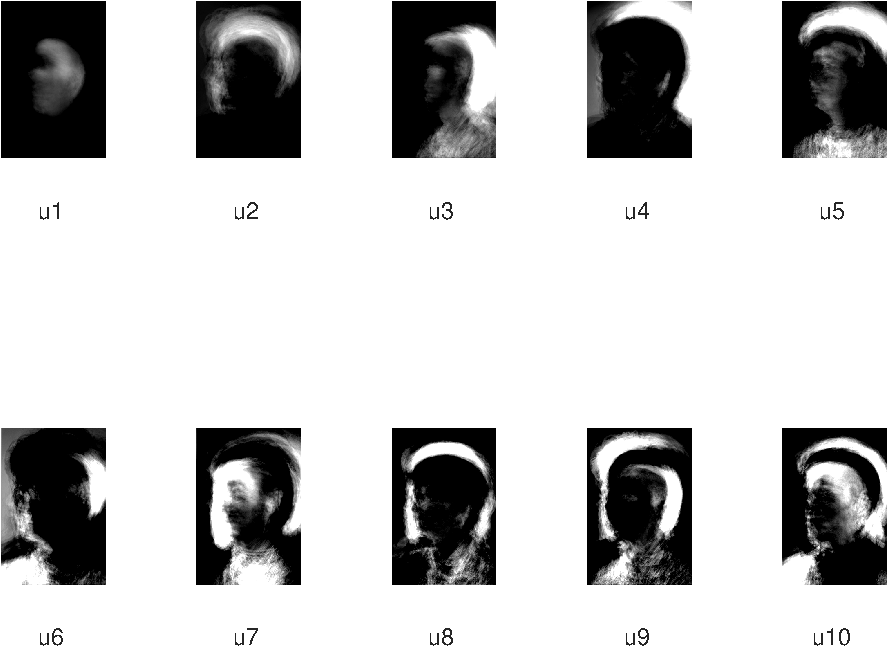
\includegraphics[height=2.5cm]{Figures/10_eigen_faces_m50deg}
\caption{$\Theta_2= -50^{\circ}$}
\end{subfigure}\vspace{5mm}
\begin{subfigure}[b]{0.4\textwidth}
	\centering
	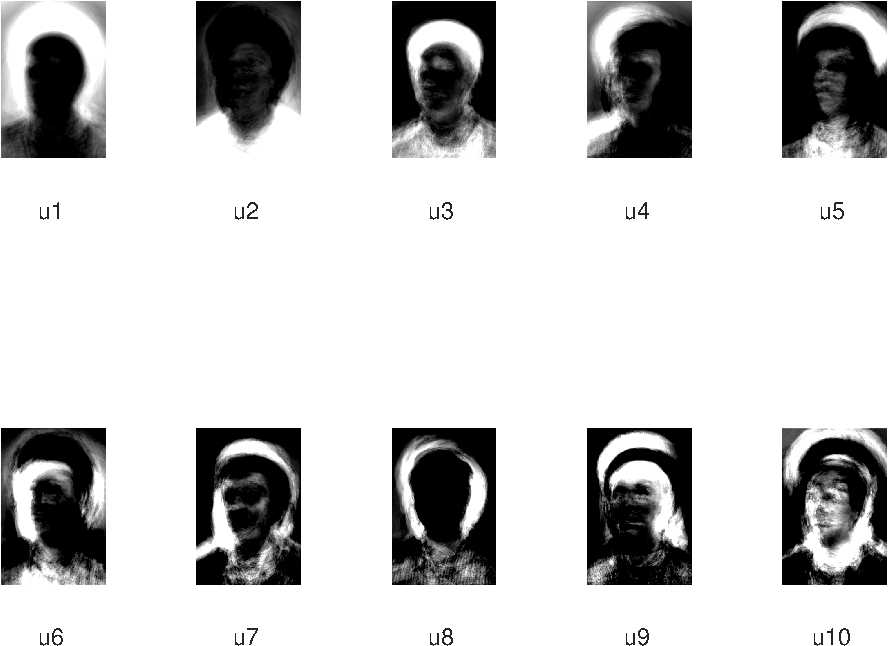
\includegraphics[height=2.5cm]{Figures/10_eigen_faces_m15deg}
\caption{$\Theta_3= -15^{\circ}$}
\end{subfigure}~
\begin{subfigure}[b]{0.4\textwidth}
	\centering
	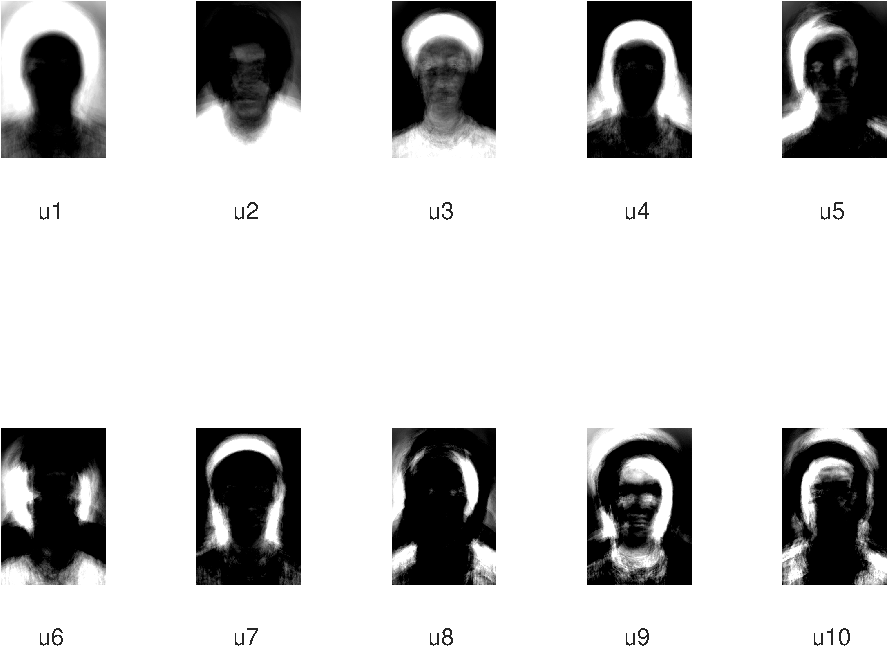
\includegraphics[height=2.5cm]{Figures/10_eigen_faces_0deg}
\caption{$\Theta_4= 0^{\circ}$}
\end{subfigure}\vspace{5mm}

\begin{subfigure}[b]{0.4\textwidth}
	\centering
	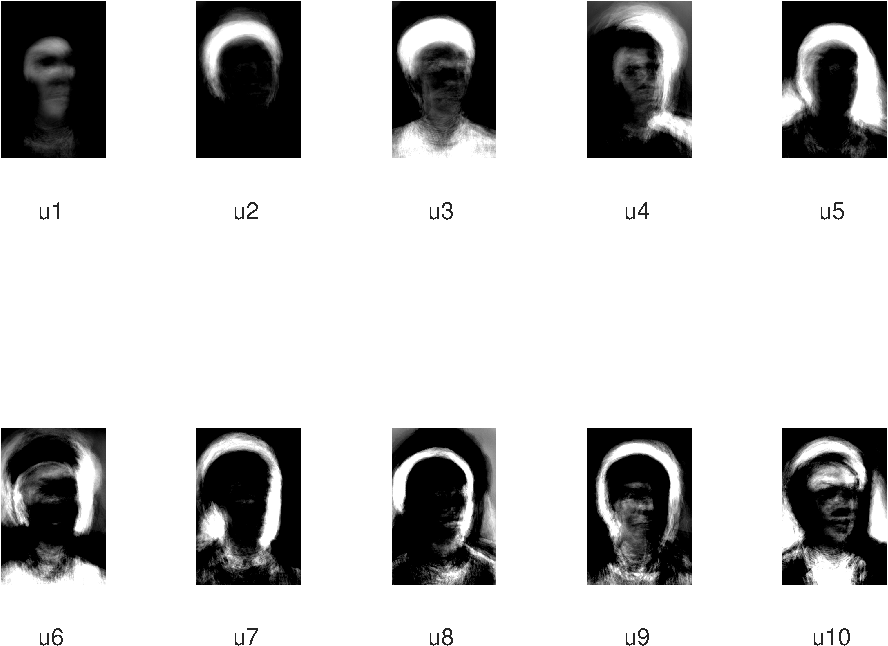
\includegraphics[height=2.5cm]{Figures/10_eigen_faces_15deg}
\caption{$\Theta_5= +15^{\circ}$}
\end{subfigure}~
\begin{subfigure}[b]{0.4\textwidth}
	\centering
	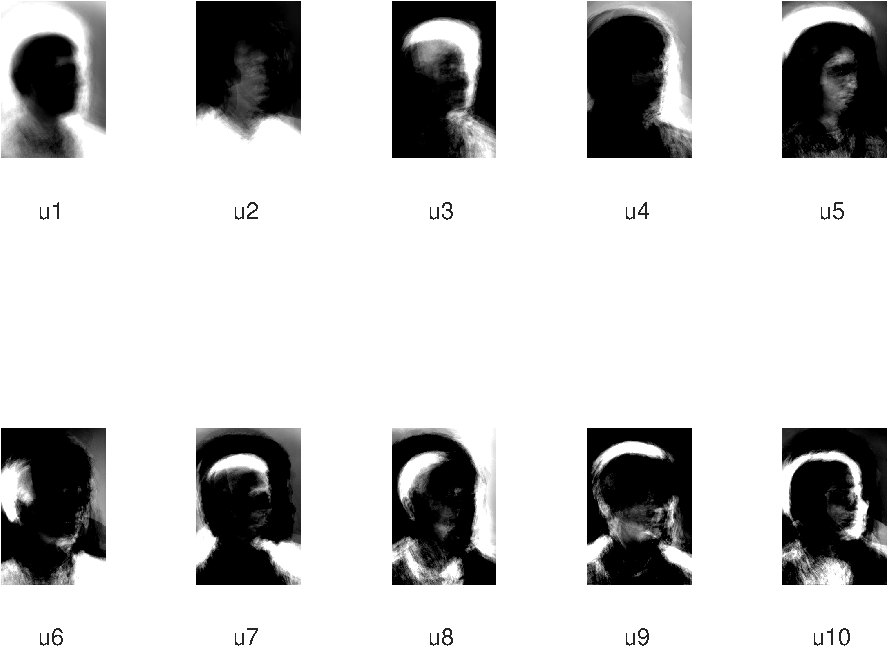
\includegraphics[height=2.5cm]{Figures/10_eigen_faces_50deg}
\caption{$\Theta_6= +50^{\circ}$}
\end{subfigure}\vspace{5mm}
\begin{subfigure}[b]{0.4\textwidth}
	\centering
	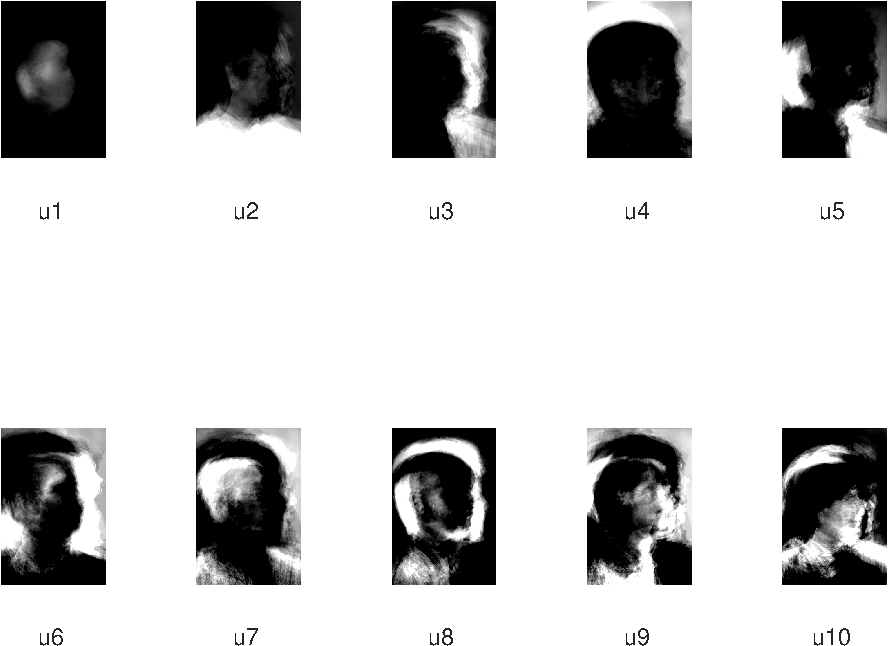
\includegraphics[height=2.5cm]{Figures/10_eigen_faces_90deg}
\caption{$\Theta_7= +90^{\circ}$}
\end{subfigure}
\caption{Top $10$ eigen faces $u_i$ for each pose class $\Theta_j$.}
\label{fig:10_eigen_faces_pose}
\end{figure}

\subsection{Pose Classification}

Using the same method that in the previous section, we will classify each testing image using nearest neighbourhood. We have to project each testing image into $7$ different space each representing one pose. We compute the nearest neighbour for one space and we take the distance value for the nearest image. Then we have $7$ possible images (each the nearest for one pose space), the minimun distance of these $7$ images is our class prediction.
The marginal error rate for with $1$, $2$, $5$, $10$, $20$, $30$, $50$, $90$, $100$, all eigen values is shown in Figure \ref{fig:error_rate_eig_pose}. The error rate is quite high because the algorithm tend to confound people when there are not the same and in the same orientation (Fig. \ref{fig:error_class_pose_eig}). All the confusion matrices are shown in Table \ref{tab:conf1}-\ref{tab:confall}. It can be seen that the more we take eigen values, more accurate we are. Many predicted poses are near the diagonal, that mean that the algorithm confound near pose (Fig. \ref{fig:error_class_pose_eig}), but recognize well when the two images has more distinct poses.

\begin{figure}
\centering
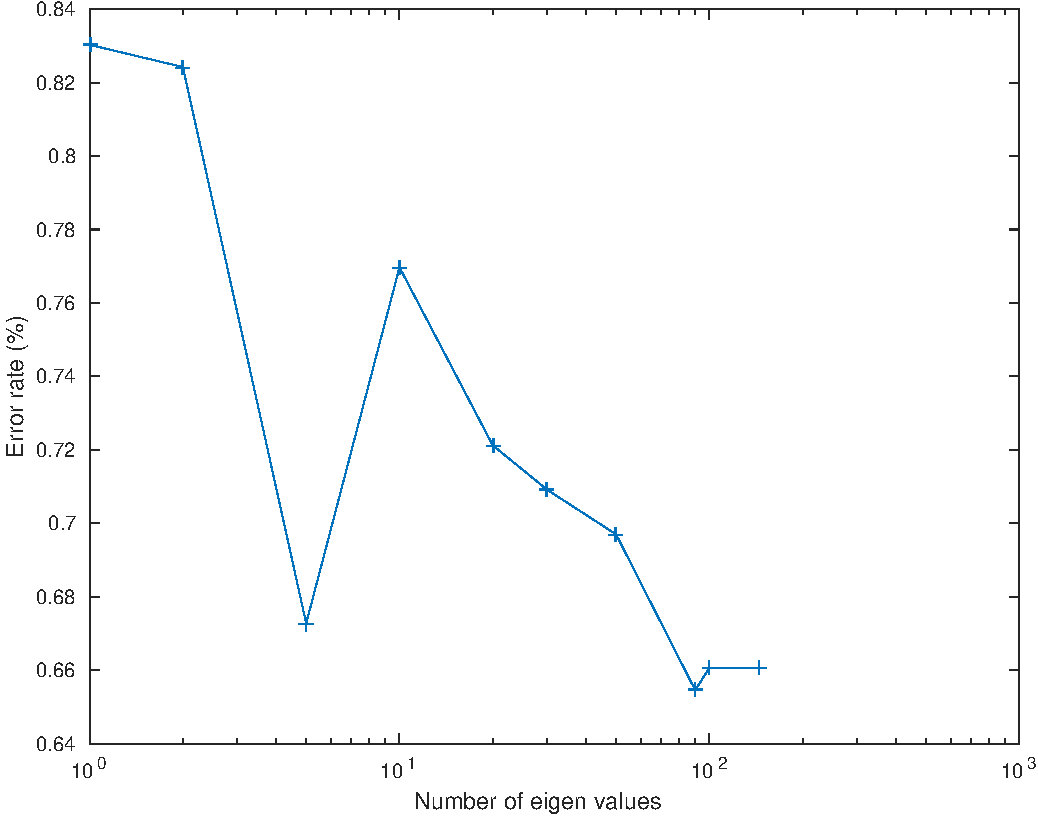
\includegraphics[height=5cm]{Figures/error_rate_eig_pose}
\caption{Error rate for eigen values. Nota : the last number of eigen values depends on the training pose set because it is not uniform, so I took an average of $150$. }
\label{fig:error_rate_eig_pose}
\end{figure}

\begin{table}
\centering
\caption{Confusion matrix for $1$ eigen value.}
\label{tab:conf1}
\begin{tabular}{@{}r|ccccccc@{}}
\toprule
Prediction & \multicolumn{1}{r}{$\Theta_1$} & \multicolumn{1}{r}{$\Theta_2$} & \multicolumn{1}{r}{$\Theta_3$} & \multicolumn{1}{r}{$\Theta_4$} & \multicolumn{1}{r}{$\Theta_5$} & \multicolumn{1}{r}{$\Theta_6$} & \multicolumn{1}{r}{$\Theta_7$} \\ \midrule
$\Theta_1$ & 3                              & 2                              & 1                              & 2                              & 2                              & 4                              & 2                              \\
$\Theta_2$ & 2                              & 3                              & 1                              & 2                              & 5                              & 5                              & 5                              \\
$\Theta_3$ & 0                              & 3                              & 3                              & 7                              & 3                              & 5                              & 1                              \\
$\Theta_4$ & 0                              & 2                              & 10                             & 4                              & 6                              & 6                              & 4                              \\
$\Theta_5$ & 3                              & 2                              & 2                              & 6                              & 6                              & 5                              & 3                              \\
$\Theta_6$ & 1                              & 1                              & 3                              & 4                              & 5                              & 5                              & 3                              \\
$\Theta_7$ & 1                              & 3                              & 2                              & 4                              & 5                              & 4                              & 4                              \\ \midrule
Actual     & \multicolumn{1}{l}{}           & \multicolumn{1}{l}{}           & \multicolumn{1}{l}{}           & \multicolumn{1}{l}{}           & \multicolumn{1}{l}{}           & \multicolumn{1}{l}{}           & \multicolumn{1}{l}{}           \\ \cmidrule(r){1-1}
\end{tabular}
\end{table}

\begin{table}
\centering
\caption{Confusion matrix for $2$ eigen value.}
\label{tab:conf2}
\begin{tabular}{@{}r|ccccccc@{}}
\toprule
Prediction & \multicolumn{1}{r}{$\Theta_1$} & \multicolumn{1}{r}{$\Theta_2$} & \multicolumn{1}{r}{$\Theta_3$} & \multicolumn{1}{r}{$\Theta_4$} & \multicolumn{1}{r}{$\Theta_5$} & \multicolumn{1}{r}{$\Theta_6$} & \multicolumn{1}{r}{$\Theta_7$} \\ \midrule
$\Theta_1$ & 4                              & 1                              & 0                              & 2                              & 4                              & 4                              & 1                              \\
$\Theta_2$ & 2                              & 3                              & 4                              & 5                              & 5                              & 4                              & 0                              \\
$\Theta_3$ & 0                              & 1                              & 5                              & 6                              & 3                              & 5                              & 2                              \\
$\Theta_4$ & 0                              & 4                              & 6                              & 6                              & 10                             & 3                              & 3                              \\
$\Theta_5$ & 0                              & 1                              & 4                              & 7                              & 4                              & 6                              & 5                              \\
$\Theta_6$ & 0                              & 2                              & 2                              & 2                              & 6                              & 3                              & 7                              \\
$\Theta_7$ & 0                              & 5                              & 2                              & 5                              & 4                              & 3                              & 4                              \\ \midrule
Actual     & \multicolumn{1}{l}{}           & \multicolumn{1}{l}{}           & \multicolumn{1}{l}{}           & \multicolumn{1}{l}{}           & \multicolumn{1}{l}{}           & \multicolumn{1}{l}{}           & \multicolumn{1}{l}{}           \\ \cmidrule(r){1-1}
\end{tabular}
\end{table}

\begin{table}
\centering
\caption{Confusion matrix for $5$ eigen value.}
\label{tab:conf5}
\begin{tabular}{@{}r|ccccccc@{}}
\toprule
Prediction & \multicolumn{1}{r}{$\Theta_1$} & \multicolumn{1}{r}{$\Theta_2$} & \multicolumn{1}{r}{$\Theta_3$} & \multicolumn{1}{r}{$\Theta_4$} & \multicolumn{1}{r}{$\Theta_5$} & \multicolumn{1}{r}{$\Theta_6$} & \multicolumn{1}{r}{$\Theta_7$} \\ \midrule
$\Theta_1$ & 4                              & 7                              & 2                              & 2                              & 0                              & 1                              & 0                              \\
$\Theta_2$ & 4                              & 10                             & 4                              & 4                              & 1                              & 0                              & 0                              \\
$\Theta_3$ & 0                              & 2                              & 7                              & 8                              & 4                              & 1                              & 0                              \\
$\Theta_4$ & 2                              & 0                              & 6                              & 10                             & 10                             & 2                              & 2                              \\
$\Theta_5$ & 0                              & 0                              & 1                              & 13                             & 7                              & 5                              & 1                              \\
$\Theta_6$ & 0                              & 0                              & 2                              & 2                              & 4                              & 5                              & 9                              \\
$\Theta_7$ & 0                              & 0                              & 1                              & 2                              & 0                              & 9                              & 11                             \\ \midrule
Actual     & \multicolumn{1}{l}{}           & \multicolumn{1}{l}{}           & \multicolumn{1}{l}{}           & \multicolumn{1}{l}{}           & \multicolumn{1}{l}{}           & \multicolumn{1}{l}{}           & \multicolumn{1}{l}{}           \\ \cmidrule(r){1-1}
\end{tabular}
\end{table}

\begin{table}
\centering
\caption{Confusion matrix for $10$ eigen value.}
\label{tab:conf10}
\begin{tabular}{@{}r|ccccccc@{}}
\toprule
Prediction & \multicolumn{1}{r}{$\Theta_1$} & \multicolumn{1}{r}{$\Theta_2$} & \multicolumn{1}{r}{$\Theta_3$} & \multicolumn{1}{r}{$\Theta_4$} & \multicolumn{1}{r}{$\Theta_5$} & \multicolumn{1}{r}{$\Theta_6$} & \multicolumn{1}{r}{$\Theta_7$} \\ \midrule
$\Theta_1$ & 1                              & 9                              & 4                              & 1                              & 0                              & 1                              & 0                              \\
$\Theta_2$ & 6                              & 6                              & 7                              & 2                              & 1                              & 1                              & 0                              \\
$\Theta_3$ & 0                              & 3                              & 9                              & 7                              & 3                              & 0                              & 0                              \\
$\Theta_4$ & 0                              & 1                              & 9                              & 8                              & 12                             & 1                              & 1                              \\
$\Theta_5$ & 0                              & 1                              & 0                              & 13                             & 7                              & 5                              & 1                              \\
$\Theta_6$ & 0                              & 0                              & 1                              & 1                              & 8                              & 2                              & 10                             \\
$\Theta_7$ & 0                              & 0                              & 0                              & 2                              & 1                              & 15                             & 5                              \\ \midrule
Actual     & \multicolumn{1}{l}{}           & \multicolumn{1}{l}{}           & \multicolumn{1}{l}{}           & \multicolumn{1}{l}{}           & \multicolumn{1}{l}{}           & \multicolumn{1}{l}{}           & \multicolumn{1}{l}{}           \\ \cmidrule(r){1-1}
\end{tabular}
\end{table}

\begin{table}
\centering
\caption{Confusion matrix for $20$ eigen value.}
\label{tab:conf20}
\begin{tabular}{@{}r|ccccccc@{}}
\toprule
Prediction & \multicolumn{1}{r}{$\Theta_1$} & \multicolumn{1}{r}{$\Theta_2$} & \multicolumn{1}{r}{$\Theta_3$} & \multicolumn{1}{r}{$\Theta_4$} & \multicolumn{1}{r}{$\Theta_5$} & \multicolumn{1}{r}{$\Theta_6$} & \multicolumn{1}{r}{$\Theta_7$} \\ \midrule
$\Theta_1$ & 4                              & 9                              & 1                              & 0                              & 2                              & 0                              & 0                              \\
$\Theta_2$ & 8                              & 5                              & 5                              & 4                              & 1                              & 0                              & 0                              \\
$\Theta_3$ & 0                              & 3                              & 8                              & 7                              & 4                              & 0                              & 0                              \\
$\Theta_4$ & 0                              & 0                              & 6                              & 9                              & 15                             & 1                              & 1                              \\
$\Theta_5$ & 0                              & 0                              & 2                              & 13                             & 8                              & 4                              & 0                              \\
$\Theta_6$ & 0                              & 0                              & 1                              & 1                              & 8                              & 2                              & 10                             \\
$\Theta_7$ & 0                              & 1                              & 0                              & 1                              & 0                              & 11                             & 10                             \\ \midrule
Actual     & \multicolumn{1}{l}{}           & \multicolumn{1}{l}{}           & \multicolumn{1}{l}{}           & \multicolumn{1}{l}{}           & \multicolumn{1}{l}{}           & \multicolumn{1}{l}{}           & \multicolumn{1}{l}{}           \\ \cmidrule(r){1-1}
\end{tabular}
\end{table}

\begin{table}
\centering
\caption{Confusion matrix for $30$ eigen value.}
\label{tab:conf30}
\begin{tabular}{@{}r|ccccccc@{}}
\toprule
Prediction & \multicolumn{1}{r}{$\Theta_1$} & \multicolumn{1}{r}{$\Theta_2$} & \multicolumn{1}{r}{$\Theta_3$} & \multicolumn{1}{r}{$\Theta_4$} & \multicolumn{1}{r}{$\Theta_5$} & \multicolumn{1}{r}{$\Theta_6$} & \multicolumn{1}{r}{$\Theta_7$} \\ \midrule
$\Theta_1$ & 4                              & 9                              & 1                              & 0                              & 2                              & 0                              & 0                              \\
$\Theta_2$ & 9                              & 6                              & 5                              & 3                              & 0                              & 0                              & 0                              \\
$\Theta_3$ & 0                              & 3                              & 8                              & 7                              & 4                              & 0                              & 0                              \\
$\Theta_4$ & 0                              & 0                              & 7                              & 8                              & 15                             & 1                              & 1                              \\
$\Theta_5$ & 0                              & 0                              & 2                              & 12                             & 8                              & 5                              & 0                              \\
$\Theta_6$ & 0                              & 0                              & 0                              & 1                              & 9                              & 2                              & 10                             \\
$\Theta_7$ & 0                              & 0                              & 1                              & 0                              & 1                              & 9                              & 12                             \\ \midrule
Actual     & \multicolumn{1}{l}{}           & \multicolumn{1}{l}{}           & \multicolumn{1}{l}{}           & \multicolumn{1}{l}{}           & \multicolumn{1}{l}{}           & \multicolumn{1}{l}{}           & \multicolumn{1}{l}{}           \\ \cmidrule(r){1-1}
\end{tabular}
\end{table}

\begin{table}
\centering
\caption{Confusion matrix for $50$ eigen value.}
\label{tab:conf50}
\begin{tabular}{@{}r|ccccccc@{}}
\toprule
Prediction & \multicolumn{1}{r}{$\Theta_1$} & \multicolumn{1}{r}{$\Theta_2$} & \multicolumn{1}{r}{$\Theta_3$} & \multicolumn{1}{r}{$\Theta_4$} & \multicolumn{1}{r}{$\Theta_5$} & \multicolumn{1}{r}{$\Theta_6$} & \multicolumn{1}{r}{$\Theta_7$} \\ \midrule
$\Theta_1$ & 5                              & 9                              & 1                              & 0                              & 1                              & 0                              & 0                              \\
$\Theta_2$ & 10                             & 6                              & 4                              & 3                              & 0                              & 0                              & 0                              \\
$\Theta_3$ & 0                              & 3                              & 9                              & 6                              & 4                              & 0                              & 0                              \\
$\Theta_4$ & 0                              & 0                              & 6                              & 9                              & 15                             & 2                              & 0                              \\
$\Theta_5$ & 0                              & 0                              & 1                              & 14                             & 8                              & 4                              & 0                              \\
$\Theta_6$ & 0                              & 0                              & 0                              & 1                              & 9                              & 2                              & 10                             \\
$\Theta_7$ & 0                              & 0                              & 1                              & 1                              & 0                              & 10                             & 11                             \\ \midrule
Actual     & \multicolumn{1}{l}{}           & \multicolumn{1}{l}{}           & \multicolumn{1}{l}{}           & \multicolumn{1}{l}{}           & \multicolumn{1}{l}{}           & \multicolumn{1}{l}{}           & \multicolumn{1}{l}{}           \\ \cmidrule(r){1-1}
\end{tabular}
\end{table}

\begin{table}
\centering
\caption{Confusion matrix for $90$ eigen value.}
\label{tab:conf90}
\begin{tabular}{@{}r|ccccccc@{}}
\toprule
Prediction & \multicolumn{1}{r}{$\Theta_1$} & \multicolumn{1}{r}{$\Theta_2$} & \multicolumn{1}{r}{$\Theta_3$} & \multicolumn{1}{r}{$\Theta_4$} & \multicolumn{1}{r}{$\Theta_5$} & \multicolumn{1}{r}{$\Theta_6$} & \multicolumn{1}{r}{$\Theta_7$} \\ \midrule
$\Theta_1$ & 5                              & 9                              & 1                              & 0                              & 1                              & 0                              & 0                              \\
$\Theta_2$ & 9                              & 8                              & 4                              & 2                              & 0                              & 0                              & 0                              \\
$\Theta_3$ & 0                              & 3                              & 10                             & 6                              & 3                              & 0                              & 0                              \\
$\Theta_4$ & 0                              & 0                              & 6                              & 12                             & 13                             & 1                              & 0                              \\
$\Theta_5$ & 0                              & 0                              & 0                              & 14                             & 9                              & 4                              & 0                              \\
$\Theta_6$ & 0                              & 0                              & 0                              & 1                              & 9                              & 3                              & 9                              \\
$\Theta_7$ & 0                              & 0                              & 0                              & 2                              & 0                              & 11                             & 10                             \\ \midrule
Actual     & \multicolumn{1}{l}{}           & \multicolumn{1}{l}{}           & \multicolumn{1}{l}{}           & \multicolumn{1}{l}{}           & \multicolumn{1}{l}{}           & \multicolumn{1}{l}{}           & \multicolumn{1}{l}{}           \\ \cmidrule(r){1-1}
\end{tabular}
\end{table}

\begin{table}
\centering
\caption{Confusion matrix for $100$ eigen value.}
\label{tab:conf100}
\begin{tabular}{@{}r|ccccccc@{}}
\toprule
Prediction & \multicolumn{1}{r}{$\Theta_1$} & \multicolumn{1}{r}{$\Theta_2$} & \multicolumn{1}{r}{$\Theta_3$} & \multicolumn{1}{r}{$\Theta_4$} & \multicolumn{1}{r}{$\Theta_5$} & \multicolumn{1}{r}{$\Theta_6$} & \multicolumn{1}{r}{$\Theta_7$} \\ \midrule
$\Theta_1$ & 5                              & 9                              & 1                              & 0                              & 1                              & 0                              & 0                              \\
$\Theta_2$ & 9                              & 8                              & 4                              & 2                              & 0                              & 0                              & 0                              \\
$\Theta_3$ & 0                              & 3                              & 10                             & 6                              & 3                              & 0                              & 0                              \\
$\Theta_4$ & 0                              & 0                              & 6                              & 12                             & 13                             & 1                              & 0                              \\
$\Theta_5$ & 0                              & 0                              & 1                              & 14                             & 8                              & 4                              & 0                              \\
$\Theta_6$ & 0                              & 0                              & 0                              & 1                              & 9                              & 3                              & 9                              \\
$\Theta_7$ & 0                              & 0                              & 0                              & 2                              & 0                              & 11                             & 10                             \\ \midrule
Actual     & \multicolumn{1}{l}{}           & \multicolumn{1}{l}{}           & \multicolumn{1}{l}{}           & \multicolumn{1}{l}{}           & \multicolumn{1}{l}{}           & \multicolumn{1}{l}{}           & \multicolumn{1}{l}{}           \\ \cmidrule(r){1-1}
\end{tabular}
\end{table}

\begin{table}
\centering
\caption{Confusion matrix for all eigen value.}
\label{tab:confall}
\begin{tabular}{@{}r|ccccccc@{}}
\toprule
Prediction & \multicolumn{1}{r}{$\Theta_1$} & \multicolumn{1}{r}{$\Theta_2$} & \multicolumn{1}{r}{$\Theta_3$} & \multicolumn{1}{r}{$\Theta_4$} & \multicolumn{1}{r}{$\Theta_5$} & \multicolumn{1}{r}{$\Theta_6$} & \multicolumn{1}{r}{$\Theta_7$} \\ \midrule
$\Theta_1$ & 5                              & 9                              & 1                              & 0                              & 1                              & 0                              & 0                              \\
$\Theta_2$ & 11                             & 7                              & 4                              & 0                              & 0                              & 0                              & 1                              \\
$\Theta_3$ & 0                              & 3                              & 11                             & 4                              & 4                              & 0                              & 0                              \\
$\Theta_4$ & 0                              & 0                              & 10                             & 9                              & 12                             & 1                              & 0                              \\
$\Theta_5$ & 0                              & 0                              & 1                              & 13                             & 9                              & 4                              & 0                              \\
$\Theta_6$ & 0                              & 0                              & 0                              & 1                              & 9                              & 3                              & 9                              \\
$\Theta_7$ & 0                              & 0                              & 0                              & 0                              & 0                              & 11                             & 12                             \\ \midrule
Actual     & \multicolumn{1}{l}{}           & \multicolumn{1}{l}{}           & \multicolumn{1}{l}{}           & \multicolumn{1}{l}{}           & \multicolumn{1}{l}{}           & \multicolumn{1}{l}{}           & \multicolumn{1}{l}{}           \\ \cmidrule(r){1-1}
\end{tabular}
\end{table}

The Figure \ref{fig:error_class_pose_eig} shows three missclassified images and three good classification. We wee that when the training image has the same face in testing it's easier for the algorithm to find the good position.

\begin{figure}
\centering
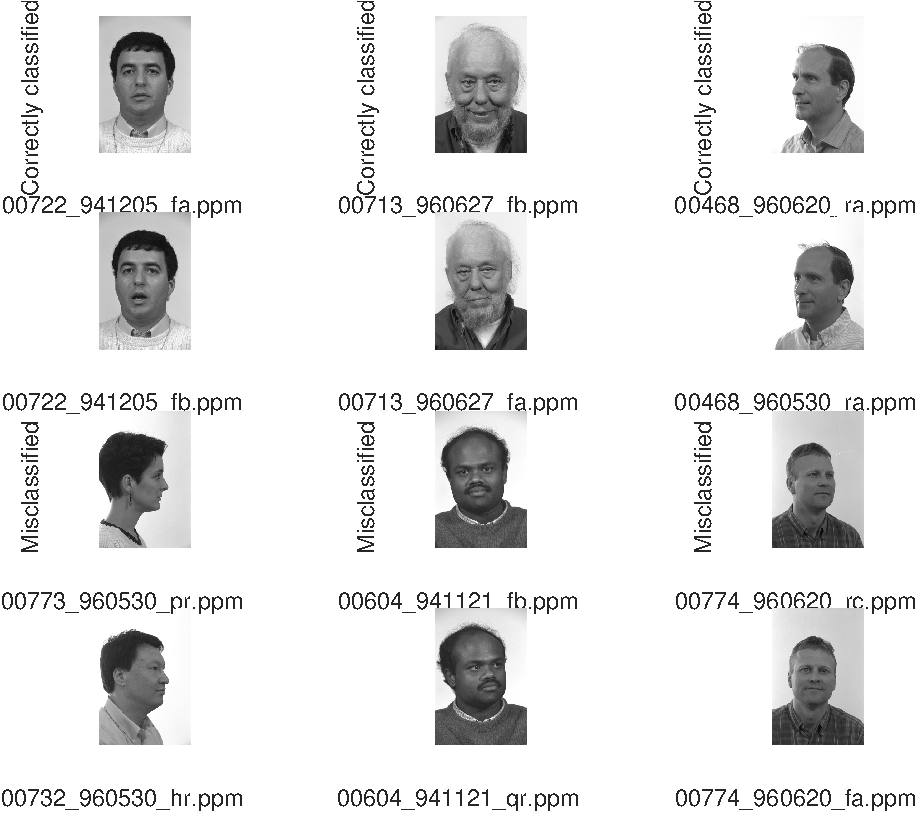
\includegraphics[height=5cm]{Figures/error_class_pose_eig}
\caption{Missclassified and good pose classified examples.}
\label{fig:error_class_pose_eig}
\end{figure}

\subsection{Probabilistic Pose Classification}

The classification can be also computed using a bayesian rule. Assuming that the data $d$ (pixels) are well fitted to the model $m$ (eigen values), the probability for one class $l$ given an image $I$ is :

\begin{equation}
p(l=k|I)=\frac{p(I|l=k)~p(l=k)}{p(I)}
\end{equation}

Because $p(l=k|I) ~\alpha~p(I|l=k)p(l=k)$, to assign a label to a given image we will assume the following assumption :

\begin{equation}
\max p(l=k|I) \simeq \max p(I|l=k)
\end{equation}

The likelihood $p(I|l=k)$ for each subject $k$ will be approximated by a multivariate gaussian on all images for each pose with $50$ eigen weights with the covariance $\Sigma$ $50$ by $50$ and mean $\mu$. Using $50$ values, the recognition rate is $27\%$ (Tab. \ref{tab:conf50pose}) which is lower than $35\%$ for the nearest neighbour. When we take not enough training data, the eigen weights are not well distributed and there are computation problem with the covariance. The Figure \ref{fig:proba_eig_pose} shows the distribution of the previous images and we see that it tends to be uniform.
\begin{table}
\centering
\caption{Confusion matrix for 50 eigen value.}
\label{tab:conf50pose}
\begin{tabular}{@{}r|ccccccc@{}}
\toprule
Prediction & \multicolumn{1}{r}{$\Theta_1$} & \multicolumn{1}{r}{$\Theta_2$} & \multicolumn{1}{r}{$\Theta_3$} & \multicolumn{1}{r}{$\Theta_4$} & \multicolumn{1}{r}{$\Theta_5$} & \multicolumn{1}{r}{$\Theta_6$} & \multicolumn{1}{r}{$\Theta_7$} \\ \midrule
$\Theta_1$ & 7                              & 3                              & 2                              & 0                              & 0                              & 1                              & 3                              \\
$\Theta_2$ & 8                              & 5                              & 3                              & 7                              & 0                              & 0                              & 0                              \\
$\Theta_3$ & 6                              & 3                              & 4                              & 8                              & 0                              & 0                              & 1                              \\
$\Theta_4$ & 12                             & 1                              & 3                              & 10                             & 4                              & 0                              & 2                              \\
$\Theta_5$ & 10                             & 1                              & 1                              & 3                              & 3                              & 5                              & 4                              \\
$\Theta_6$ & 7                              & 0                              & 4                              & 1                              & 5                              & 4                              & 1                              \\
$\Theta_7$ & 3                              & 0                              & 3                              & 0                              & 6                              & 0                              & 11                             \\ \midrule
Actual     & \multicolumn{1}{l}{}           & \multicolumn{1}{l}{}           & \multicolumn{1}{l}{}           & \multicolumn{1}{l}{}           & \multicolumn{1}{l}{}           & \multicolumn{1}{l}{}           & \multicolumn{1}{l}{}           \\ \cmidrule(r){1-1}
\end{tabular}
\end{table}

\begin{figure}
\centering
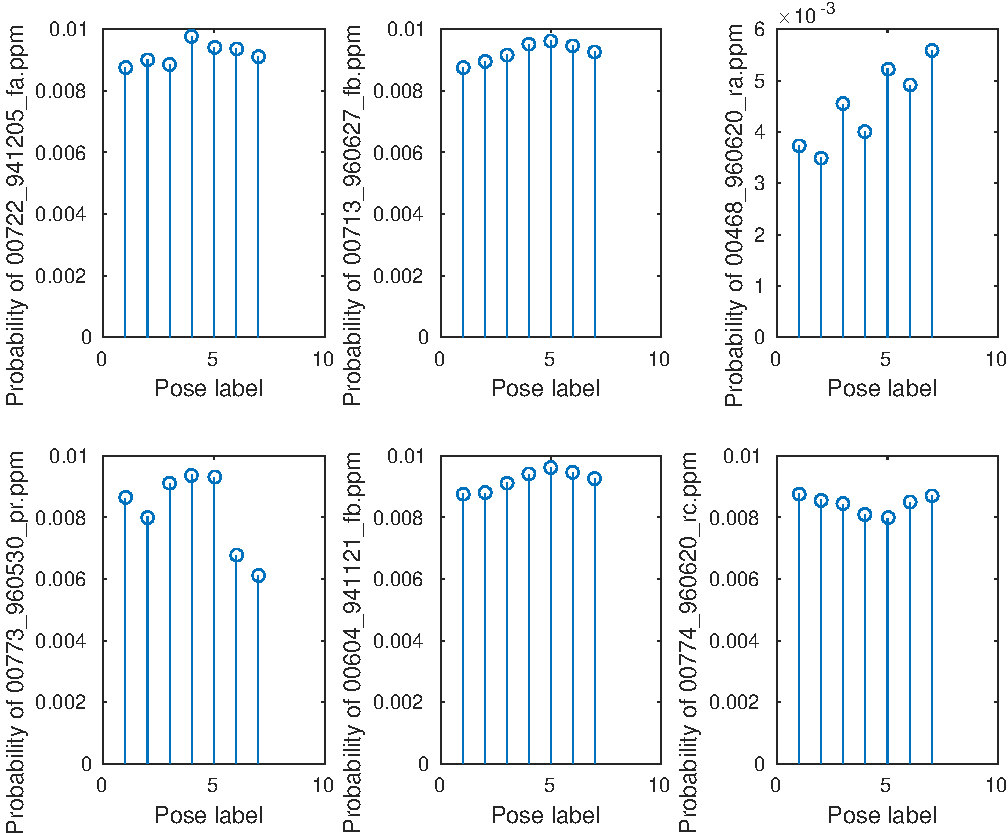
\includegraphics[height=5cm]{Figures/proba_eig_pose}
\caption{Likelihoods of missclassified and good pose classified examples.}
\label{fig:proba_eig_pose}
\end{figure}

\section{Conclusion}

The goal of this assignment was to perform image classification using PCA. We saw two approaches on two problems : Nearest neighbour and Bayes with face and pose classification. 
The neighbouring approach does not need assumptions in the data, however it just give us a strict label without more information. In the other hand, the bayesian approach need one assumption and a multivariate gaussian assumption was made. It is difficult to modelise the likelihoods of the subjects if there is no precision about the underlying model, but it has the advantage to give more information than NN. \par
Face classification gives better recognition rate $(\simeq 70\%)$ than pose recognition $(\simeq 35\%)$. I explain this because the eigen faces are more sensitive to the human face, than to its position. The PCA has difficulties to be consistent in general, here with angles but also with lighting condition or scale.

{\small
\bibliographystyle{splncs03}
\bibliography{assignment2}
}

\end{document}
